% Run this command from vim
% :setlocal makeprg=cd\ report\ &&\ pdflatex\ -interaction=batchmode\ main.tex\ &&\ xdg-open\ main.pdf
% then to compile and open the file just run :make (or press F8)

\documentclass[a4paper, titlepage]{article}
\newcommand{\Punit}[0]{\frac{\unit{\mega\electronvolt}}{c^2 \unit{\femto\meter}}}
\newcommand{\Sh}[0]{Schwarzschild }

\usepackage[T1]{fontenc}
\usepackage[utf8]{inputenc}
\usepackage[italian]{babel}
%\usepackage[hashEnumerators,smartEllipses]{markdown}
\usepackage{mathtools}
\usepackage{siunitx} % Load siunitx first
\usepackage{physics} % Load physics after siunitx
%\usepackage{amsmath} %mathtools loads amsmath too!!
\usepackage{amssymb}
\usepackage[overload]{empheq}
\usepackage{listings}
\usepackage{tabularx}
\usepackage{textcomp}
\usepackage{multirow}
\usepackage{multicol}
\usepackage{booktabs}
\usepackage{graphicx}
\usepackage{floatflt}
\usepackage{epsfig}
\usepackage{pstricks}
\usepackage{subcaption}
\usepackage[labelfont=bf, font=scriptsize]{caption}
\usepackage[italian]{varioref}
\usepackage[suftesi,write]{frontespizio}
\usepackage{xcolor}
\usepackage{caption}
\usepackage{pgfplots}
\usepackage{comment}
\usepackage{bm}            % special bold-math package. usge: \bm{mathsymbol}
\usepackage{array}
\usepackage{lipsum}
\usepackage{csquotes}
\usepackage{biblatex}
%\addbibresource{sample-paper.bib}
\usepackage[colorlinks=true]{hyperref}  % this package should be added after all others.
\pgfplotsset{compat=1.16}
\usepackage[text={15.5cm,23.5cm},centering,heightrounded]{geometry}
\DeclareCaptionType{eq_caption}[Equazione][Elenco delle equazioni]

\definecolor{mygreen}{rgb}{0,0.6,0}
\definecolor{mygray}{rgb}{0.5,0.5,0.5}
\definecolor{mymauve}{rgb}{0.58,0,0.82}

\lstset{ 
  backgroundcolor=\color{white},   % choose the background color; you must add \usepackage{color} or \usepackage{xcolor}; should come as last argument
  basicstyle=\footnotesize,        % the size of the fonts that are used for the code
  breakatwhitespace=false,         % sets if automatic breaks should only happen at whitespace
  breaklines=true,                 % sets automatic line breaking
  captionpos=b,                    % sets the caption-position to bottom
  commentstyle=\color{mygreen},    % comment style
  deletekeywords={...},            % if you want to delete keywords from the given language
  escapeinside={\%*}{*)},          % if you want to add LaTeX within your code
  extendedchars=true,              % lets you use non-ASCII characters; for 8-bits encodings only, does not work with UTF-8
  firstnumber=1,                   % start line enumeration with line 1000
  frame=single,	                 % adds a frame around the code
  keepspaces=true,                 % keeps spaces in text, useful for keeping indentation of code (possibly needs columns=flexible)
  keywordstyle=\color{blue},       % keyword style
  %language=Octave,                % the language of the code
  morekeywords={*,...},            % if you want to add more keywords to the set
  numbers=left,                    % where to put the line-numbers; possible values are (none, left, right)
  numbersep=5pt,                   % how far the line-numbers are from the code
  numberstyle=\tiny\color{mygray}, % the style that is used for the line-numbers
  rulecolor=\color{black},         % if not set, the frame-color may be changed on line-breaks within not-black text (e.g. comments (green here))
  showspaces=false,                % show spaces everywhere adding particular underscores; it overrides 'showstringspaces'
  showstringspaces=false,          % underline spaces within strings only
  showtabs=false,                  % show tabs within strings adding particular underscores
  stepnumber=1,                    % the step between two line-numbers. If it's 1, each line will be numbered
  stringstyle=\color{mymauve},     % string literal style
  tabsize=2,	                   % sets default tabsize to 2 spaces
  title=\lstname                   % show the filename of files included with \lstinputlisting; also try caption instead of title
}

%\begin{frontespizio}
    \Universita{Trento} % CTT
    \Logo{Figures/logo_unitn} % CTT
    \Divisione{Fisica Computazionale} % CTT
    \Corso[Laurea Triennale]{Fisica} % CTT, a meno che non cambi la denominazione del corso
    \Annoaccademico{2023-2024}
    \Titoletto{Progetto Finale} % CTT
    \Titolo{Calcolo redshift nell'emissione di fotoni da una stella di neutroni\\ }
    \Sottotitolo{\today}
    \Candidato[227552]{Federico De Paoli, \textsf {federico.depaoli@studenti.unitn.it}}
    \NRelatore{Docente}{} % CTT
    \Relatore{Prof. Alessandro Roggero} % CTT, a meno che non sia cambiato il Prof.
\end{frontespizio}
\IfFileExists{\jobname-frn.pdf}{}{%
\immediate\write18{pdflatex \jobname-frn}} % ASSOLUTAMENTE CTT, è il comando che materialmente vi genera il frontespizio.

\newpage



\begin{document}

\tableofcontents
\newpage

\section{Introduzione}
Studiamo la stabilità delle stelle di neutroni in regime relativistico considerando 3 possibili equazioni di stato per la materia.
Una volta risolte le equazioni è possibile ottenere l'espressione del potenziale gravitazione della stella e calcolare l'effetto sulla radiazione emessa dalla stella.


Viene calcolata la radianza per ogni stella a 3 distanze diverse e la potenza totale di emissione in funzione della distanza dalla stella.
Viene quindi calcolata la temperatura apparente delle 3 stelle più massive in funzione di quella effettiva e poi viene studiata la temperatura apparente in funzione della pressione centrale della stella.

\section{Stabilità}

Le equazioni che descrivono la stabilità di una stella in funzione della massa ($m$) e della pressione ($P$) sono quelle di Tolman-Oppenheimer-Volkoff
\begin{subequations}
    \begin{align}[left = {\empheqlbrace}]
        \dv[]{P(r)}{r} &= - G \frac{m(r) \epsilon (r)}{r^2 c^2} \left(1 + \frac{P(r)}{\epsilon (r)} \right) \left(\ + \frac{4 \pi r^3 P(r)}{m(r) c^2} \right) \left(1 - \frac{2 G m(r)}{r c^2} \right)^{-1} \label{eq:P_corr} \\
        \dv[]{m(r)}{r} &= 4 \pi r^2 \frac{\epsilon (r)}{c^2} \label{eq:m_corr} \\
        \dv[]{\Phi(r)}{r} &= - \frac{1}{P(r) + \epsilon (r)} \dv[]{P(r)}{r} \label{eq:Phi_corr}
    \end{align}
    \label{eq:sistema_corr}
\end{subequations}

Dove la terza equazione è l'equazione disaccoppiata e descrive il potenziale gravitazionale della stella.
Usiamo 3 diverse densità di energia per la materia della stella (eq. \ref{eq:energia23} viene presa con due coppie di valori diversi di $\Gamma$ e $K$):
\begin{subequations}
\begin{align}
    \epsilon_1 (n) &= a \left( \frac{n}{n_0} \right) ^{\alpha} + b \left( \frac{n}{n_0} \right) ^{\beta} \label{eq:energia1} \\
    \epsilon_{2/3} (n) &= \mu c^2n+Kc^2n^\Gamma \label{eq:energia23}
\end{align}
\end{subequations}
\begin{equation}
    \text{con} \quad a = 13.4 \unit{\mega\electronvolt\per\femto\cubic\meter} \ , \quad
    \alpha = 0.514, \quad
    b = 5.62 \unit{\mega\electronvolt\per\femto\cubic\meter} \ , \quad
    \beta = 2.436 \ , \quad
    n_0 = 0.16 \unit{\per\femto\cubic\meter}
\end{equation}

dove $n$ è la densità numerica, $\mu$ la massa di una singola particella e quindi $\rho = \mu n$ è la densità di massa.


Visto che la densità di energia è in funzione di $\rho$ e le incognite del sistema \ref{eq:sistema_corr} sono $P$ e $m$ possiamo scrivere la densità di energia in funzione di $P$ e $m$ partendo dalla relazione termodinamica

\begin{subequations}
    \label{eq:eps(r)}
    \begin{align}[left = {P = - \dv[]{E}{V} \Rightarrow \empheqlbrace}]
        P &= (\alpha - 1) a \left( \frac{n}{n_0} \right)^{\alpha} + (\beta - 1) b \left( \frac{n}{n_0} \right)^{\beta} && \text{per } \epsilon_1 \label{eq:eps(r)1} \\
        n &= \left( \frac{P}{K(\Gamma - 1) c^2} \right)^{1 / \Gamma} && \text{per } \epsilon_{1/2} \label{eq:eps(r)23}
    \end{align}
\end{subequations}

Nel primo caso (eq. \ref{eq:eps(r)1}) non è stato possibile invertire l'equazione per trovare $n$ in funzione di $P$ e $m$ quindi utilizzeremo un metodo numerico per trovare $n$ di volta in volta.

Facciamo le seguenti sostituzioni per rendere le variabili adimensionali e con valori più vicini a 0.

\begin{equation*}
    m=M_0\hat m, \quad 
    r=R_0\hat r, \quad 
    P=P_0\hat P, \quad
    \rho=\rho_0 \hat{\rho}, \quad
    K = \hat{K}\frac{\mu^\Gamma}{\rho_0^{\Gamma-1}},
\end{equation*}

\begin{subequations}
    \begin{align}[left = {\empheqlbrace}]
        \dv[]{\hat P}{\hat r} &= - \frac{(\hat P + \hat{\epsilon})(\hat m + \hat r^3 \hat P)}{\hat r^2-2\hat m\hat r} \label{eq:P_ad} \\
        \dv[]{\hat m}{\hat r} &= \hat r^2 \hat{\epsilon} \label{eq:m_ad} \\
        \dv[]{\Phi}{\hat r} &= - \frac{1}{\hat P + \hat{\epsilon}} \dv[]{\hat P}{\hat r} \label{eq:Phi_ad}
    \end{align}
    \label{eq:sistema_adim}
\end{subequations}

Otteniamo il sistema \ref{eq:sistema_adim} dove, grazie alle equazioni in \ref{eq:eps(r)}, $\hat m$, $\hat P$ e $\hat{\epsilon}$ sono funzioni di $\hat r$. Come valori delle costanti sono stati usati

\begin{equation}
    M_0 = 12.655756 M_\odot \quad R_0 = 20.06145 \unit{\kilo\meter} \quad \epsilon = P_0 = \rho_0 c^2 = 150.174 \Punit
    \label{eq:val_cost}
\end{equation}

Per il potenziale gravitazionale $\Phi$ si può inoltre trovare una soluzione analitica all'esterno della stella che possiamo mettere in forma adimensionale (eq. \ref{eq:Phi_ext}), dove $\hat{M}$ e $\hat R$ sono rispettivamente la massa totale e il raggio della stella in forma adimensionale.

\begin{equation}
    \Phi_\text{ext} (r) = \frac{1}{2} \log(1 - \frac{2 G M}{r c^2})
    \implies \Phi_\text{ext} (\hat r) = \frac{1}{2} \log(1 - \frac{2 \hat{M}}{\hat r}) \quad \quad \hat r \geq \hat{R}
    \label{eq:Phi_ext}
\end{equation}


\section{Curva massa raggio}
Cominciamo con il risolvere le prime due equazioni \ref{eq:P_ad} e \ref{eq:m_ad} del sistema adimensionale con il metodo \texttt{RK4} (appendice \ref{ap:RK4}).
Per il caso con equzione di stato più complessa (eq. \ref{eq:energia1}) viene risolta numericamente l'equazione \ref{eq:eps(r)1} per trovare $\rho$ da $P$ (Appendice \ref{ap:eps(r)1}).

Segliamo massa iniziale 0 e pressioni iniziali differenti in modo da trovare soluzioni con $R$ compreso tra i 3 e i 60 \unit{\kilo\meter}. Il grafico massa raggio trovato viene riportato in figura \ref{fig:MR}.

\begin{figure}[h]
        \centering
        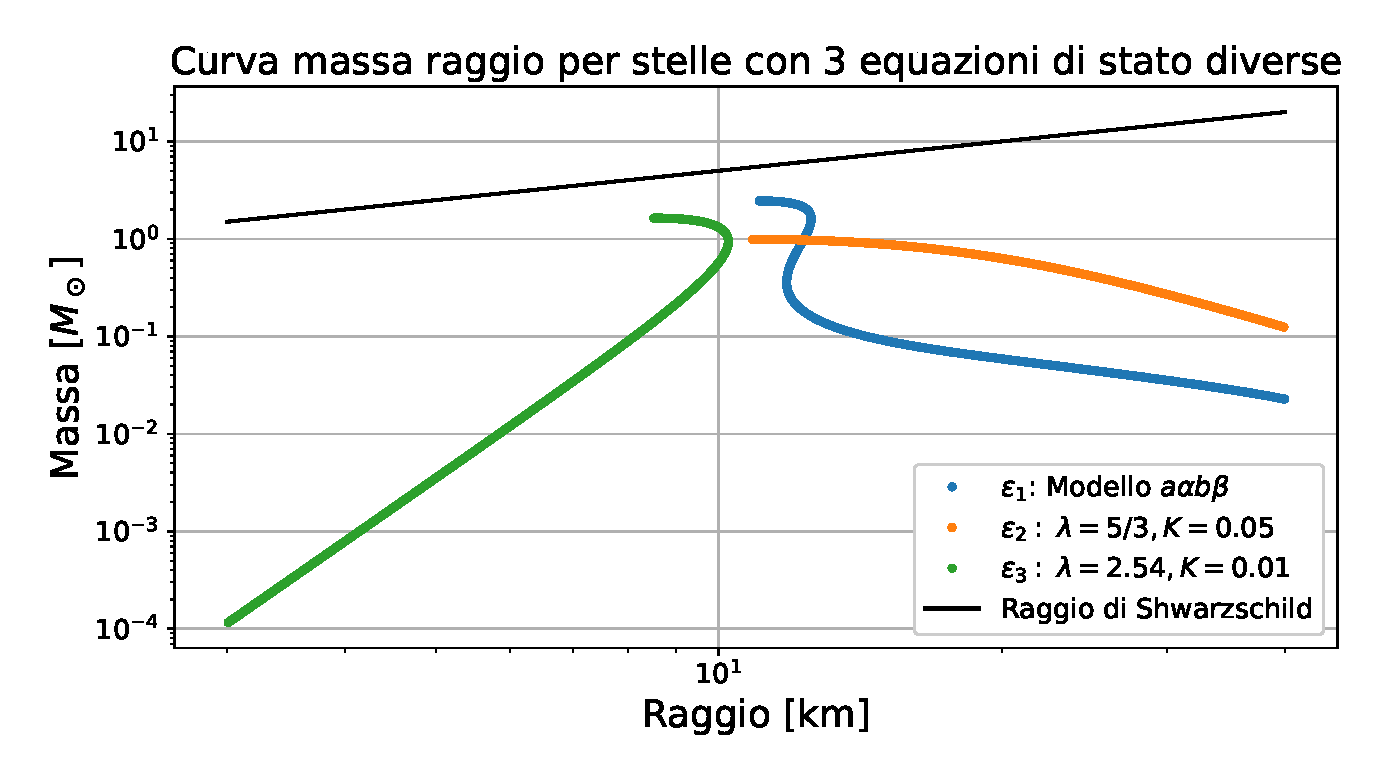
\includegraphics[width = 0.6 \textwidth]{Figures/MR.eps}
        \caption{Curva massa raggio per stelle di equzioni di stato $\epsilon_{1/2/3}$. La prima equazione di stato, quella più realistica, prevede stelle di neutroni più massive.}
        \label{fig:MR}
\end{figure}

Durante l'esecuzione del programma abbiamo inoltre smesso di incrementare la pressione centrale iniziale quando la condizione di stabilità $\dv[]{M}{r} > 0$ veniva meno.

Notiamo subito che con l'equazione di stato \ref{eq:energia1} il modello prevede stelle con massa e raggio maggiore rispetto al limite previsto dagli altri modelli.

I valori della stella più massiva per ogni equazione di stato diversa vengono riportati nella tabella \ref{tab:Mgrosso}.

\begin{table}[h!]
    \centering
    \begin{tabular}{c|c|c|c}
        & $P_0~[\Punit]$ & $R~[\unit{\kilo\meter}]$ & $M~[M_\odot]$ \\
         \hline
         $\epsilon_1$ & 43.31065 & 59.03824 & 14.29963 \\
         \hline
         $\epsilon_2$ & 217.0675 & 10.90280 & 0.9252994 \\
         \hline
         $\epsilon_3$ & 947.5339 & 8.559218 & 1.528782 \\
    \end{tabular}
    \caption{Valori della pressione iniziale $P_0$, massa totale $M$ e raggio $R$ della stella più massiva per ogni equazione di stato utilizzata.}
    \label{tab:Mgrosso}
\end{table}


\section{Potenziale gravitazionale}

Come mostrato nel sistema \ref{eq:sistema_corr}, l'equzione che determina il potenziale gravitazionale è disaccoppiata dalle altre due e, per $r \geq R$, può anche essere risolta analiticamente.
Utilizzando le equazioni \ref{eq:Phi_ad} e \ref{eq:Phi_ext} possiamo trovare l'espressione generale per il potenziale all'interno della stella riportata in eq. \ref{eq:Phi_int1}.

\begin{equation}
    \Phi_\text{int} (\hat r) =
    \Phi_\text{ext} (\hat R) - \int_{\hat r}^{\hat R} \dv[]{\Phi}{x} \;\mathrm{d}x =
    \frac{1}{2} \log(1 - \frac{2 \hat M}{\hat R}) + \int_{\hat r}^{\hat R} \frac{1}{\hat P (x) + \hat \epsilon (x)} \dv[]{\hat P (x)}{x} \;\mathrm{d}x
    \label{eq:Phi_int1}
\end{equation}

dove siamo stati attenti a rendere $\Phi (r)$ continuo per ogni $r \geq 0$ usando il valore di $\Phi_\text{ext}$ in $\hat R$. Infine sostituendo alla derivata della pressione l'espressione in \ref{eq:P_ad} otteniamo

\begin{equation}
    \Phi_\text{int} (\hat r) =
    \frac{1}{2} \log(1 - \frac{2 \hat{M}}{\hat R}) + \int_{\hat r}^{\hat R} \frac{\hat m (x) + x^3 \hat P (x)}{2 \hat m (x) x - x^2}  \;\mathrm{d}x
    \label{eq:Phi_int2}
\end{equation}

Dati i valori di $\hat P (\hat r)$ e $\hat m (\hat r)$ che si ottengono risolvendo le equazioni di stabilità possiamo quindi disegnare il grafico del potenziale gravitazionale, mostrato in figura \ref{fig:Phi}.

\begin{figure}[h]
    \centering
    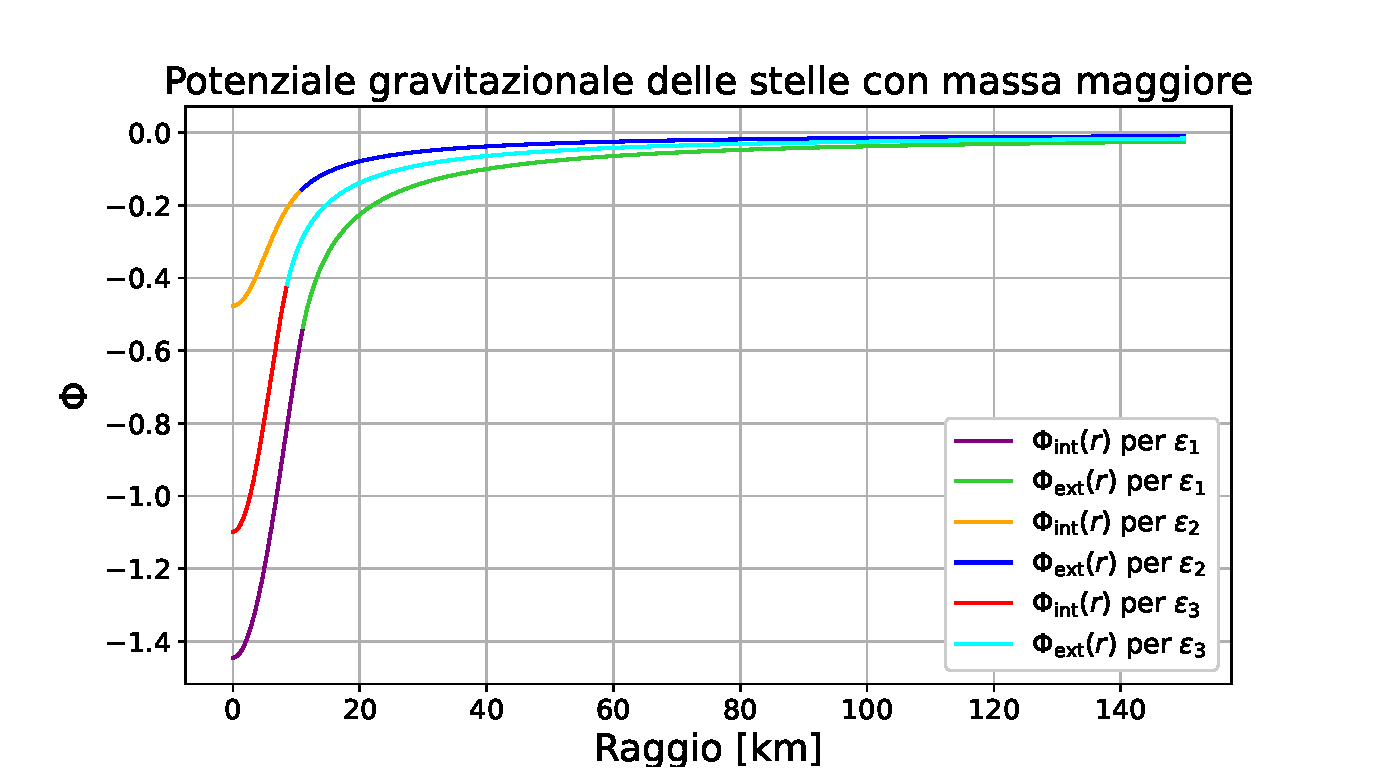
\includegraphics[width = \textwidth]{Figures/Phi.eps}
    \caption{Grafico del potenziale gravitazionale all'interno e all'esterno della stella. Per $r < R$ è stato ottenuto integrando con il metodo dei trapezzi l'eq. \ref{eq:Phi_int2}, per $r \geq R$ è stata plottata l'eq. \ref{eq:Phi_ext}}
    \label{fig:Phi}
\end{figure}

Vediamo dalla figura \ref{fig:Phi} che in tutti e 3 i casi $\Phi (r)$ è continuo, grazie alla condizione imposta.

Il potenziale $\Phi$ (che fa parte del termine $e^{\Phi (r)} c^2 \mathrm{d}t^2$ della metrica $\mathrm{d}s^2$, che descrive la geometria dello spazio vicino alla stella) assume un andamento famigliare: raggiunge valori più bassi per le stelle più massive al diminuire di $r$ e tende a 0 per $r$ grandi.




\newpage
\section{Radianza}

In metrica di \Sh un fotone emesso a distanza $r$ con frequenza $\nu_\text{em}$ viene ricevuto da un osservatore a distanza $r'$ con una frequeza $\nu_\text{ric}$ data da

\begin{equation}
    \frac{\nu_\text{ric}}{\nu_\text{em}} = e^{\Phi (r) - \Phi (r')} \, .
\label{eq:redshift}
\end{equation}

Dove $\Phi (r)$ è propio il potenziale gravitazionale mostrato in figura \ref{fig:Phi}.

La radianza di una stella si può esprimere con l'equazione di Plank per il corpo nero

\begin{equation}
    B(\nu, T) = \frac{2 h \nu ^3}{c^2} \frac{1}{e^{h \nu / (k_B T)} - 1}
    \label{eq:rad}
\end{equation}

dove $T$ è la temperatura della stella e $h$ la costante di Plank.





















%%%%%%%%%%%%%%%%%%%%%%%%%%%%%%%%%%%%%%%%%%%%%%%%%%%%%%%%%%%%%%%%%%%%%%%%%%%%%%%%%%%%%%%%%
%%%%%%%%%%%%%%%%%%%%%%%%                APPENDICI               %%%%%%%%%%%%%%%%%%%%%%%%% 
%%%%%%%%%%%%%%%%%%%%%%%%%%%%%%%%%%%%%%%%%%%%%%%%%%%%%%%%%%%%%%%%%%%%%%%%%%%%%%%%%%%%%%%%%

\newpage
\appendix

\section{RK4} \label{ap:RK4}
Codice con cui è stato implementato il metodo \texttt{RK4}. \texttt{fun\_P()} e \texttt{fun\_m()} sono le funzioni presenti a destra dell'uguale nella prima e nella seconda riga del sistema \ref{eq:sistema_adim}.

\begin{lstlisting}[language=C]
void rungeKutta4(double h, double r, double *P, double *m, int tipo_politropica){

    double k1, k2, k3, k4, l1, l2, l3, l4;

    k1 = h * fun_m(r, *P, tipo_politropica);
    l1 = h * fun_P(r, *P, *m, tipo_politropica);

    k2 = h * fun_m(r + h / 2, *P + l1 / 2, tipo_politropica);
    l2 = h * fun_P(r + h / 2, *P + l1 / 2, *m + k1 / 2, tipo_politropica);

    k3 = h * fun_m(r + h / 2, *P + l2 / 2, tipo_politropica);
    l3 = h * fun_P(r + h / 2, *P + l2 / 2, *m + k2 / 2, tipo_politropica);

    k4 = h * fun_m(r + h, *P + l3, tipo_politropica);
    l4 = h * fun_P(r + h, *P + l3, *m + k3, tipo_politropica);

    *m += (k1 + 2 * k2 + 2 * k3 + k4) / 6;
    *P += (l1 + 2 * l2 + 2 * l3 + l4) / 6;
}
\end{lstlisting}

\section{Risoluzione numerica di $\hat P (\rho)$} \label{ap:eps(r)1}

Quando si calcola il valore della derivata di $P$ o $m$ ad un dato $r$ serve anche il valore dell'energia interna, infatti
\begin{lstlisting}[language=C]
// fun_m = r^3 E
double fun_m(double r, double P, int tipo_politropica){
    return r * r * fun_E(P, tipo_politropica);
}


// fun_P = - (P + E)(m + r^3 P)/(r^2 - 2mr)
double fun_P(double r, double P, double m, int tipo_politropica){
    if (m == 0)
        return 0;
    return (P + fun_E(P, tipo_politropica)) * (m + pow(r, 3) * P) / ((2 * m - r) * r);
}
\end{lstlisting}
Dove la funzione \texttt{fun\_E()} è definita come
\begin{lstlisting}[language=C]
double fun_E(double P, int tipo_politropica){
    // Politropica quasi realistica (a*rho^alpha + b*rho^beta)
    if (tipo_politropica == 0){
        double rho = findRho(P);
        return A * pow(rho, ALPHA) + B * pow(rho, BETA);
    }

    double lambda, K;

    // Politropiche semplici
    if (tipo_politropica == 1){
        lambda = 5. / 3.;
        K = 0.05;
    } else if (tipo_politropica == 2){
        lambda = 2.54;
        K = 0.01;
    } else {
        printf("Tipo politropica non riconosciuto\n");
        return 0;
    }

    double a1 = P / (lambda - 1);
    return a1 + pow(a1 / K, 1. / lambda);
}
\end{lstlisting}

Per le politropiche semplici (eq. \ref{eq:energia23}) abbiamo potuto trovare un'espressione analitica per $\rho (P)$ (eq. \ref{eq:eps(r)23}). L'energia può quindi essere calcolata in modo diretto come viene fatto nelle righe 22-23 del codice sopra riportato.

Per la politropica \ref{eq:energia1}, la relazione tra $\rho$ e $P$ che si trova è data in \ref{eq:eps(r)1}, che riportiamo

\begin{equation}
        P = (\alpha - 1) a \left( \frac{n}{n_0} \right)^{\alpha} + (\beta - 1) b \left( \frac{n}{n_0} \right)^{\beta} \ .
        \label{ap:eq:1}
\end{equation}

Data una certa pressione $P$ bisopgna quindi risolvere numericamente l'equazione per trovare il valore $n$ che la soddisfa. Per fare ciò utiliziamo la funzione \texttt{findRho()} così definita

\begin{lstlisting}[language=C]
double findRho(double P){

    // Cominciamo prima con il metodo di Newton-Raphson
    if (P > 0.01){

        double rho = pow(P / (BETA1 * B), 1 / BETA);    // buona approx. iniziale
        while (fabs(P - P_of_rho(rho)) > 1e-6){
            rho -= (P_of_rho(rho) - P) / DP_of_rho(rho);
        }
        return rho;
    }

    // Per P piccoli meglio usare bisezione
    double rho_sx = 0.7, rho_dx = 1.;
    double rho = (rho_sx + rho_dx) / 2;
    while (fabs(P - P_of_rho(rho)) > 1e-6){
        if (P_of_rho(rho) > P)
            rho_dx = rho;
        else
            rho_sx = rho;
        rho = (rho_sx + rho_dx) / 2;
    }
    return rho;
}
\end{lstlisting}

dove \texttt{P\_odf\_rho()} e \texttt{DP\_of\_rho()} sono rispettivamente la funzione \ref{ap:eq:1} e la sua derivata. In questo modo possiamo sempre trasformare $\epsilon (\rho)$ in $\epsilon (P)$.

\end{document}



































%% Snippets cos I'm too lazy to set the Lsp the right way


%\begin{figure}[h]
%    \begin{minipage}{0.48\textwidth}
%        \centering
%        \includegraphics[width = \textwidth]{Figures/Figure_rho0.91.png}
%        \caption{Coordinate x e y delle particelle.
%        Sullla stessa fiura sono state plottate le posizioni delle particelle per ogni instante temporale successivo a \texttt{nsteps/2} e per ogni valore di $z$.
%        A $\rho = 0.91$ le particelle sono disposte in modo disordinato. \\}
%        \label{fig:rho0.91}
%    \end{minipage}
%    \hspace{0.015\textwidth}    
%    \begin{minipage}{0.48\textwidth}
%        \centering
%        \includegraphics[width = \linewidth]{Figures/Figure_rho0.97.png}
%        \caption{Coordinate x e y delle particelle.
%        Sullla stessa fiura sono state plottate le posizioni delle particelle per ogni instante temporale successivo a \texttt{nsteps/2} e per ogni valore di $z$.
%        A $\rho = 0.97$ la struttura \texttt{BCC} è ben visibile e per ogni posizione si vede quanto può oscillare una particelle.}
%        \label{fig:rho0.97}
%    \end{minipage}
%\end{figure}


%\begin{table}[h!]
%    \centering
%    \begin{tabular}{c|c|c|c}
%          & SC & BCC & FCC \\
%         \hline
%         $N$ & $n^3$ & $2 n^3$ & $4 n^3$ \\
%         \hline
%         $a$ & $\rho^{-1/3}$ & $\left( \frac{\rho}{2} \right)^{-1/3}$ & $\left( \frac{\rho}{4} \right)^{-1/3}$ \\
%    \end{tabular}
%    \caption{Dipendenza di $N$ e $a$ da $n$ e $\rho$}
%    \label{tab:my_label}
%\end{table}
